\documentclass{article}
\usepackage{amssymb}
\usepackage{amsmath}
\usepackage{bbm}
\usepackage{graphicx}
\usepackage{color}
\usepackage{fancyref}
\usepackage{cite}
\usepackage{hyperref}
\usepackage{float}


\sloppy
\definecolor{lightgray}{gray}{0.5}
\setlength{\parindent}{0pt}

\title{\textbf{Nonlinear Anderson Acceleration for implicit Runge Kutta integrators}}
\author{Giacomo Garegnani \\ {Supervisors: Andrea Di Blasio and Prof. Assyr Abdulle}}
\date{\today}

\begin{document}
\maketitle

% INTRODUCTION ==============================================================================================================================================================
\begin{section}{Introduction}
The Runge-Kutta integrators for Ordinary Differential Equations (ODEs) are a class of numerical methods with a various range of features. In particular, some Runge-Kutta integrators have a good stability behaviour independently from the chosen step size, property that defines the class of the $A$-stable methods. Moreover, there exist some $A$-stable integrators which do not produce oscillations on the numerical solution, the $L$-stable integrators. These features are of the utmost importance when one has to integrate a system of ODEs which is stiff, i.e., it is characterized by a Jacobian whose eigenvalues have a negative real part which is large in absolute value, as instable numerical methods cause diverging solutions. It has been shown that is not possible to build an explicit method that is $A$-stable, and, if the scope is integrating a stiff equation, explicit methods could require very small step sizes in order to be stable. On the other hand, many implicit methods are $A$-stable and eventually $L$-stable, as in the case of the Radau IIA integrators \cite{HW}. However implicit methods require the solution of a nonlinear system at each time step, so it is important to choose a good solver of nonlinear equations at an implementation phase. In fact, it is possible to show that using fixed point iterations often spoils the stability behaviour of the method, and the majority of the codes implementing implicit Runge-Kutta integrators use the Newton method for this purpose. In fact the Newton method converges for every choice of an initial guess which is sufficiently close to the solution, disrgarding the features of the equation if it is smooth enough. The disadvantage of the Newton method is that it requires the Jacobian of the function defining the system of ODEs, which could be difficult to compute or expensive to approximate if the size of the system is large. Moreover, it requires the solution of a linear system defined by the Jacobian, which is computationally expensive if the system is large and if it does not have particular sparsity or simmetry features. In this work we will analyze the Anderson Acceleration method for nonlinear systems \cite{WALNI,SAAD}, which is an acceleration of the fixed point iterations method, when inserted in the frame of implicit Runge-Kutta integrators. \\
The outline of the work is the following. \\
In section 2 the Anderson Acceleration method is presented together with its features.\\
Then, in section 3, the method is applied to linear diagonal stiff systems of ODEs. In fact, Anderson Acceleration is equivalent to GMRES \cite{WALNI} when applied to linear fixed point problems, so in this case the method has a typical behaviour. \\
In section 4, a strategy to implement Runge Kutta methods using Anderson Acceleration is presented in the general case of a nonlinear system of ODEs. We present the results given by the Implicit Euler method, the Implicit Trapezoidal method and the Radau IIA of third order when implemented with Anderson Acceleration. The chosen test problems are three classical examples of stiff equations, the Brussellator problem, the HIRES reaction and the Van der Pol oscillator. The performances of those implicit methods are furthermore compared to the results provided by two classic explicit methods with extended stability, the Runge Kutta Chebyshev of first and second order. A further explanation of the features of those problems, together with numerical results, could be found in \cite{HW,JC,HAIR}, while an exhaustive derivation and theoretical results for the Runge Kutta Chebyshev methods are presented in \cite{HW}.
\end{section}

\begin{section}{Anderson Acceleration method}
\begin{subsection}{Definition}
The Anderson Acceleration (AA) is an acceleration method for nonlinear fixed point problems. Given the equation
\begin{equation}
	y = G(y),
\end{equation}
the method can be implemented as follows

\noindent\rule{8cm}{0.6pt}

\noindent \textbf{anderson}($y_0\in\mathbb{R}^n,G:\mathbb{R}^n \rightarrow \mathbb{R}^n,m,n_{max}\in\mathbb{N}\setminus\{0\}$\\
1. \indent $y_1 = G(y_0); f_0 = G(y_0) - y_0; k = 2$; \\
2. \indent \textbf{until} convergence \textbf{or} $k = n_{max}$ \textbf{do} \\
3. \indent \indent \quad $m_k = min(m,k)$ \\
4. \indent \indent \quad $f_k = G(y_k) - y_k$ \\
5. \indent \indent \quad $F_k = \begin{pmatrix} f_{k-m_k+1} \cdots f_{k} \end{pmatrix} \in \mathbb{R}^{m_k\times n}$ \\
6. \indent \indent \quad $\alpha^k = \underset{\alpha \in \mathbb{R}^{m_k} : \sum_{i=1}^{m_k}\alpha_i = 1}{\arg\min} \| F_k \alpha \|_2$ \\
7. \indent \indent \quad $y_{k+1} = \sum_{j=0}^{m_k}\alpha_j^k G(y_{k-m_k+j})$ \\
8. \indent \indent \quad $k = k + 1$ \\
9. \indent \textbf{end}

\noindent\rule{8cm}{0.6pt}

The first iteration of the method is a fixed point iteration. From the second iteration onwards, the method takes into account the previous guesses of the solution for computing the next guess of the solution of problem (1). The value of $m$ has to be provided by the user. In practice, there are two possible choices for $m$. One can choose a small value, typically $m=2,3$, thus considering only the directly previous iterations for the computation of the next guess of the solution. Otherwise, a different choice is to set $m$ such that $m_k = k \; \mbox{for all } k \leq n_{max}$, where $n_{max}$ is the maximum number of iterations that the user let the method perform (practically, one can input the value $m = n_{max}$ or impose $m_k = k$ in line 4 of the pseudo-code above). In other words, at every iteration the method computes the next guess considering all the previous guesses. In this work only this second case is treated, as for Runge-Kutta methods the value $n_{max}$ is small (typically $n_{max} \leq 5$). In fact, AA is performed for every time step of the Runge-Kutta method, so the computational cost related to the nonlinear solver ought not to be exceeding the computational cost of the Runge-Kutta method itself. Furthermore, AA requires additional function evaluations that could be spoiling the performance of the integrator of the ODE. \par
As far as the stopping criterion is concerned, there are as well two possible choices. One choice could be controlling the Euclidean norm of the difference between two consecutive iterates. This choice could arise a problem if the scope is checking the number of iterations the method performs to fulfill a given tolerance, since an acceptable solution could be refused only because the previous iteration is far in norm from the current one. The other choice is controlling the norm of the residual associated to the current guess. In this work the second strategy is preferred, as the aim is showing if in a fixed number of iterations AA converges to the fixed point. \par
Finally, the last concern arose by the method is the minimization problem of line 6. The vector  $\alpha^k$ can be computed in \texttt{Matlab} using the built-in routine \texttt{fmincon}(), that finds the solution of a nonlinear constrained minimization problem. In this work, $\alpha^k$ is computed by solving the min-square solution of the following linear system
\begin{equation*}
	\begin{pmatrix}F_1 & \cdots & F_{m_k} \\ 1 & \cdots & 1 \end{pmatrix}\alpha^k = \begin{pmatrix} 0 \\ \vdots \\ 0 \\ 1 \end{pmatrix}.
\end{equation*}
There are other ways to implement AA. In particular, it is possible to reformulate the minimization problem in order to have an unconstrained minimization problem, which could be solved using the QR Housolder factorization or the SVD factorization. Further details can be found in \cite{SAAD}. However, the implementation of the method from the pseudo-code is quite straightforward, and is not the main purpose of this work.
\end{subsection}

% LINEAR AA ============================================================================================================================================== 
\begin{subsection}{Linear case}\label{subsec:linear}
Let us consider the case in which $G(y)$ is a linear function. In this case, the fixed point problem becomes
\begin{equation*}
	y = G(y) = Ay + b, \quad A \in \mathbb{R}^{n\times n}, \quad b \in \mathbb{R}^{n}.
\end{equation*} 
It is possible to show that in this case AA without truncation (i.e. $m = n_{max}$) is equivalent to the GMRES method \cite{WALNI} applied to the linear system 
\begin{equation*}
	(I - A)y = b,
\end{equation*}
where I is the identity matrix of size $n$. In particular, if $n$ is the size of the nonlinear system, AA converges to the exact solution in $n+1$ steps, which consist of the first fixed point step and $n$ other additional steps. Let us show this property analytically for the case in which $n = 1$, i.e.
\begin{equation*}
	y = G(y) = a + by, \; a,b,y \in \mathbb{R}.
\end{equation*} 
Given $y_0$, set $y_1 = G(y_0)$. Then the minimization problem of line 6. in the AA algorithm at the second iteration is
\begin{equation*}
 	(\alpha_1^1,\alpha_2^1) = \underset{\alpha_1 + \alpha_2 = 1}{\arg\min} |\alpha_1 f_0 + \alpha_2 f_1|,  
\end{equation*}
where
\begin{equation*}
	 f_0 = y_0 - G(y_0), \; f_1 = y_1 - G(y_1).
\end{equation*}
It is possible to find $\alpha_1^1,\alpha_2^1$ such that $\alpha_1^1f_0 + \alpha_2^1f_1 = 0$ and $\alpha_1^1 + \alpha_2^1 = 1$. The coefficients are given by
\begin{equation*}
	\alpha_1^1 = -\frac{f_1}{f_0 - f_1}, \quad \alpha_2^1 = \frac{f_0}{f_0 - f_1}.
\end{equation*}
Computing $y_2 = \alpha_1^1 G(y_0) + \alpha_2^1 G(y_1)$ one finds
\begin{equation*}
	y_2 = -\frac{a}{b-1} \implies y_2 = a + by_2 = G(y_2),
\end{equation*}
so after 2 steps of the algorithm the solution provided by AA is exact. This result can be extended to $n$-dimensional systems, but there are no estimations of the local error for GMRES for a general matrix. This means that the error could be large until the $n$-th iteration, dropping to zero at the last iteration. It is instead possible to show \cite{SAAD2} for a real positive definite matrix $B$ the following estimation of the residual at step $m$
\begin{equation}\label{eq:GMRESdp}
	\|r_m\| \leq \Big{(} 1 - \frac{\alpha}{\beta} \Big{)}^{m/2}\|r_0\|,
\end{equation}
where $r_0$ is the residual of the initial guess and if $M$ is the symmetric part of $B$, i.e., $M = (B + B^T)/2$
\begin{equation*}
	\alpha = (\lambda_{min}(M))^2, \quad \beta = \lambda_{max}(B^TB).
\end{equation*}
If $B$ is symmetric, then the estimation simplifies as follows
\begin{equation}\label{eq:GMRESsdp}
	\|r_m\| \leq \Big{(} 1 - \frac{\lambda_{min}(B)^2}{\lambda_{max}(B)^2} \Big{)}^{m/2}\|r_0\|.
\end{equation}
Further results for matrices with different structures can be found in \cite{SAAD2}.
\end{subsection}

\end{section}


% RUNGE KUTTA ==============================================================================================================================================
\begin{section}{Linear Systems of ODEs}
Implicit Runge Kutta methods require the solution of a nonlinear system at each time instant, which has to be solved numerically. An inadequate solver for this system can lead to timestep restrictions even for unconditionally stable methods. Let us consider Dahlquist test equation
\begin{equation*}
	y'(t) = \lambda y(t), \quad \lambda < 0, \quad |\lambda| \; \mbox{large}.
\end{equation*} 
Consider now a Runge Kutta method to solve this equation that is A-stable, for example the Implicit Euler method (IE). At each time instant, IE requires to solve the system defined by
\begin{equation*}
	y_{n+1} = y_n + h\lambda y_{n+1} = G(y_{n+1}).
\end{equation*}
Let us now pretend that this implicit equation is solved using the fixed point iterations method (FP), defined by

\noindent\rule{8cm}{0.6pt}

\noindent \textbf{fixed point}($y_0,G$) \\
1. \indent until convergence \textbf{do} \\
2. \indent \indent $y_{k+1} = G(y_k)$ \\
3. \indent \indent $k = k + 1$ \\ 
4. \indent \textbf{end}

\noindent\rule{8cm}{0.6pt}

\noindent It is known that the condition in order to have convergence of FP is of $G$ to be a contraction. In our case, this leads to the timestep restriction $ h < 1/|\lambda|$, which is even more restrictive than the timestep restriction given by the Euler Explicit method. So, if the implicit method is implemented with a fixed point solver for the nonlinear system, the stability of the method is spoilt and then an explicit method seems of more practical implementation. In order to avoid this issue, implicit Runge Kutta methods are often implemented by means of the Newton method, which ensures quadratic convergence for every function which is regular enough and for an initial guess sufficiently close to the solution. However, Newton method requires as an input the Jacobian $J$ of $G$, which is not always practical to compute, especially for large systems, and the solution of a linear system identified by $J$, which could be costly. A compromise between those two approaches can be represented by AA, as it does not require the Jacobian of $G$ and the solution of a linear system, and as it may allow larger step sizes for convergence. In fact, as it is explained in \cite{SAAD}, it is possible to show that AA is equivalent to the Broyden Quasi-Newton method. \par
The aim of this work is then studying the convergence of AA in an implicit Runge-Kutta frame. The chosen Runge-Kutta methods will always be $A$-stable, so the only issue that arises is the convergence of the nonlinear system solver. In particular, the problem could be formulated as follows 

\noindent\rule{8cm}{0.6 pt}

\textbf{Problem} \\
Given a certain tolerance $tol$ and a maximum number of iterations $n_{max}$, which is the largest step size that it is possible to choose for the implicit Runge-Kutta integrator in order to have convergence of AA up to $tol$ in $n_{max}$ iterations ?

\noindent\rule{8cm}{0.6 pt}

In the following, we present a numerical procedure which could be used in order to find numerically the solution of the problem above, and then we analyze two different cases of the application of AA to linear systems of ODEs.

% ADAPTIVITY ==============================================================================================================================================
\begin{subsection}{Adaptivity}\label{subsec:adaptlin}
Let us consider the following ODE
\begin{equation}\label{eq:ode}
	\begin{cases}
		\textbf{y}'(t) = f(t,\textbf{y}(t)), \quad \textbf{y}\in\mathbb{R}^n, f: [0,\infty] \times \mathbb{R}^n \rightarrow \mathbb{R}^n,\\
		\textbf{y}(0) =  \textbf{y}_0.
	\end{cases}
\end{equation}
Let us consider an implicit Runge-Kutta method which is A-stable, hence such that 
\begin{equation*}
 	\mathbb{C}^- \subseteq S = \{ z \in \mathbb{C}, R(z) < 1 \},
\end{equation*}
where $R(z)$ is the rational transfer function associated to the method and $S$ is the region of stability of the method. The method will require at each timestep the solution of the following fixed point problem
\begin{equation}\label{eq:fp}
	\textbf{y}_{n+1} = \phi(\textbf{y}_{n+1}; \textbf{y}_n, h_n, f),
\end{equation} 
where $\phi$ depends on the chosen Runge-Kutta method. In order to identify the step sizes for which AA converges up to a given tolerance, it is possible to use the following strategy acting on one integration step

\noindent\rule{8cm}{0.6pt}

given $\textbf{y}_n \in \mathbb{R}^n, n_{max} \in \mathbb{N}\setminus\{0\} $, $h_n \in \mathbb{R}$\\
1. compute $\textbf{y}_{n+1}$, solution of $\textbf{y}_{n+1} = \phi(\textbf{y}_{n+1}; \textbf{y}_{n}, h_{n}, f)$, using $n_{max}$ iterations of the chosen nonlinear system solver \\
2. \textbf{if} $\|\textbf{y}_{n+1} - \phi(\textbf{y}_{n+1})\| \geq tol$, $ h_{n} = h_{n} \cdot C $ \\
3. \textbf{else} \textbf{return}\\
4. \textbf{repeat} 

\noindent\rule{8cm}{0.6pt}

\noindent In the pseudocode above, $tol$ is a tolerance fixed by the user and $0 < C < 1$ is used to reduce the step size in case of failure of the nonlinear solver, and to enlarge it for the following timestep in case of success. If the aim is to identify as precisely as possible the region of convergence, a reasonable choice for $C$ is to choose it as large as possible in $(0,1)$ (e.g., $C=0.9,0.99$), provided $h_n$ large enough. The choice of $n_{max}$ has to be done carefully. It is in fact important that the computational cost given by the nonlinear solver is not too high, since the system has to be solved for each timestep. Let us denote by $h_{AA}$ the step size accepted with the above strategy. It is then the purpose of the next section finding a relation between $n_{max}$ and $h_{AA}$ for AA, especially for stiff problems, where using fixed point is not recommended due to its stepsize restriction.
\end{subsection}

% LINEAR N < NMAX ===============================================================================================================================================
\begin{subsection}{Linear case, $n < n_{max}$}\label{subsec:lin1}
Let us consider the following system of $n$ linear differential equations
\begin{equation}\label{eq:lin}
	\begin{cases}
		\textbf{y}'(t) = A\textbf{y}(t),& \textbf{y} \in \mathbb{R}^n, \; A \in \mathbb{R}^{n\times n},  \\
		\textbf{y}(0) = \mathbbm{1},	& \mathbbm{1} = \begin{pmatrix} 1 & 1 & \dots & 1 \end{pmatrix}^T \in \mathbb{R}^n.
	\end{cases}
\end{equation}
In particular, as the case of interest is mainly stiff problems, $A$ is first set as a diagonal matrix with negative entries, large in absolute value. For example let us consider the matrix defined as (in \texttt{Matlab} code)
\begin{verbatim}
A = -1000 * diag(linspace(1,5,n));
\end{verbatim}
This first experiment purpose is to verify numerically the equivalence of AA with GMRES in the linear case. As the considered problem is stiff for $t>0$, $t$ small, it is already significant considering the first timestep to verify the convergence of the nonlinear solver. Let us then apply the adaptivity strategy described in section \ref{subsec:adaptlin} with the following parameters
\begin{equation*}
	n_{max} = 2,\dots,20, \quad n = 15, \quad h_0 = 0.1, \quad tol = 10^{-6}, \quad C = 0.99,
\end{equation*}
where $h_0$ is the initial choice for the stepsize. It is expected that the values of the step sizes $h_{AA}$ chosen by the adpative procedure will be small for $n_{max}\leq n$, and they will increase with $n_{max}$, up to be exactly equal to $h_0$ for $n_{max} > n$, since for $n_{max} \geq n + 1$, AA gives the exact solution of the linear system. It is remarkable that the nonlinearity in $\phi$ as defined in section \ref{subsec:adaptlin} is only due to the nonlinearity of $f$, so in this case this result is true for every choice of a Runge-Kutta method. The following results are obtained using Implicit Euler, for which the fixed point equation is defined as
\begin{equation}\label{eq:fpIE}
	\textbf{y}_{n+1} = \phi(\textbf{y}_{n+1}; \textbf{y}_{n}, h_{n}, f) = \textbf{y}_{n} + h_nf(t_{n+1},\textbf{y}_{n+1}).
\end{equation}
In Figure \ref{fig:smallsize}, it is possible to notice that the values chosen by the method with $n_{max} \leq n$ are small if compared with the value of $h_0$, meaning that many stepsizes have been refused. 
\begin{figure}[t!]
\centering
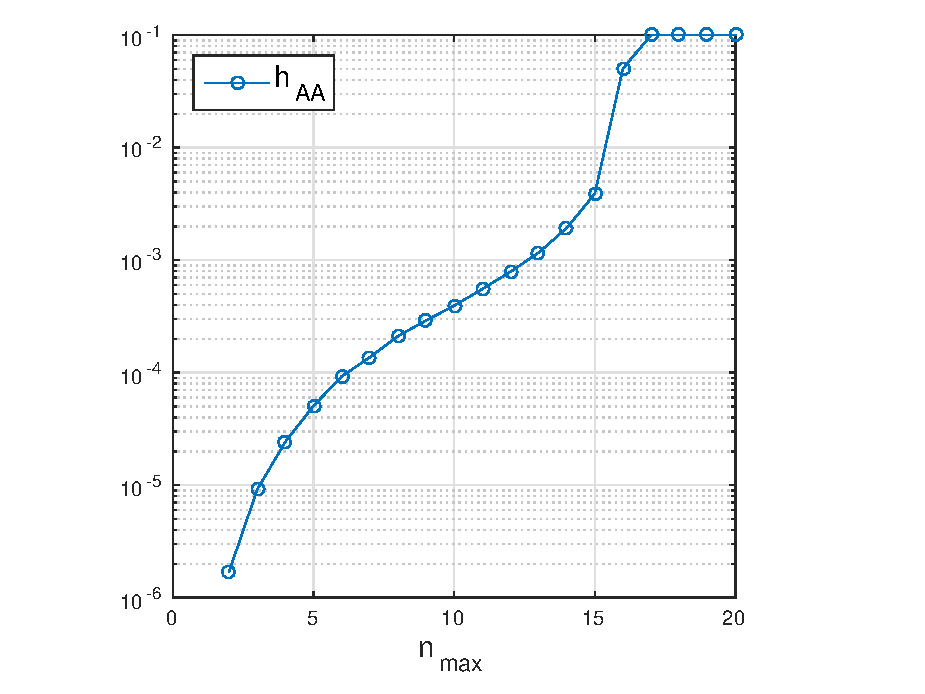
\includegraphics[width=4in]{Pictures/smallsize}
\caption{Step sizes selected by the adaptivity procedure for a system of small size solved with Implicit Euler and AA.}
\label{fig:smallsize}
\end{figure}
This is related to the claim in section \ref{subsec:linear} that GMRES, and as a consequence AA, will not provide a solution sufficiently near to the fixed point if the number of iterations is smaller than the size of the matrix. Therefore, we cannot expect $h_{AA}$ to be equal to $h_0$ in case the number of iterations performed by AA is smaller or equal to the size of the system. It is then important to remark that in certain problems, as for example in (\ref{eq:lin}), the solution is varying rapidly, and therefore a value for the step size which is too big would lead to an inaccurate solution. In the case of system (\ref{eq:lin}) it is therefore possible to conclude that AA provides the exact solution of the fixed point problem (\ref{eq:fp}) for every choice of the Runge-Kutta integrator, as long as the maximum number of iterations that AA is allowed to perform is at least equal to $n+1$, where $n$ denotes the size of the system. So, if one consider as an arresting criterion for AA only the residual, disregarding the number of iterations, the numerical solution is found exactly for any step size. This is already a remarkable gain in comparison to FP, since if for example the Implicit Euler method is used as an integrator, the following restriction on the step size is necessary for the convergence of FP
\begin{equation*}
	h < \frac{1}{|\lambda_{max}(A)|},
\end{equation*}
where $\lambda_{max}(A)$ is the eigenvalue with maximum absolute value of $A$ in system (\ref{eq:lin}). This result is independent of the number of iterations that FP is allowed to perform. 
\end{subsection}

% LINEAR N > NMAX ===============================================================================================================================================
\begin{subsection}{Linear case, $n > n_{max}$}
It is not always advisable to set $n_{max} = n+1$ for problem (\ref{eq:lin}) in order to obtain unconditioned stability for each value of the step size. In fact, if the system is big, the computational cost related to the nonlinear solver could become the most relevant for computing the solution over the timestep. It is then desirable to find an estimation of the accepted step size as function of $n_{max}$. Let us consider the Implicit Euler method, whose associated fixed point problem is defined in (\ref{eq:fpIE}). If it is applied to the system of ODEs defined in (\ref{eq:lin}), the integration over the first time step is equivalent to solving the linear system
\begin{equation*}
	(I - h_{AA}A)y_{1} = y_{0},
\end{equation*}
where $I$ is the identity matrix of size $n$. Let us consider for a matter of simplicity a matrix $A$ which is symmetric and whose real eigenvalues are such that
\begin{equation*}
	\lambda_n(A) \leq \lambda_{n-1}(A) \leq \dots \leq \lambda_1(A) < 0.
\end{equation*}
Let us denote $B = I - h_{AA}A$. $B$ is symmetric positive definite, with the eigenvalues defined by
\begin{equation*}
	\lambda_i(B) = 1 + h_{AA}|\lambda_i(A)|, \quad i = 1,\dots,n.
\end{equation*}
It is then possible to exploit the equivalence between AA and GMRES for linear systems and therefore the estimation of the residual at step $m$ (\ref{eq:GMRESsdp}), which reads 
\begin{equation}\label{eq:GMRESsdpagain}
	\|r_m\| \leq \Big{(} 1 - \frac{\lambda_{min}(B)^2}{\lambda_{max}(B)^2} \Big{)}^{m/2}\|r_0\|,
\end{equation}
where $r_0$ is the residual of the first guess of the solution. In this case
\begin{equation*}
	\lambda_{max}(B) = 1 + h_{AA}|\lambda_n(A)|, \quad \lambda_{min}(B) = 1 + h_{AA}|\lambda_1(A)|.
\end{equation*}
Furthermore, if the initial guess of the solution if $y_0$, the residual associated to it is
\begin{equation*}
	r_0 = (I - h_{AA}A)y_0 - y_0 = -h_{AA}Ay_0.
\end{equation*}
If the solution of the problem is subject to a fixed tolerance $tol$, i.e., $\|r^m\| \leq tol$, and plugging the expression of the eigenvalues and of $r_0$ into (\ref{eq:GMRESsdpagain}), it is possible to find the following expression relating the value of the step size $h_{AA}$ chosen by Implicit Euler with AA to the problem parameters
\begin{equation}\label{eq:fullestimation}
	\frac{\alpha\cdot h_{AA}^{(2+2m)/m} + \beta\cdot h_{AA}^{(2+m)/m}}{h_{AA}^2|\lambda_n|^2 + 2h_{AA}|\lambda_n| + 1} \leq \Big{(} \frac{tol}{\|Ay_0\|} \Big{)}^{2/m}, \quad \alpha,\beta \in \mathbb{R},
\end{equation}	
where the constants $\alpha$ and $\beta$ are given by
\begin{equation*}
	\alpha = |\lambda_n|^2 - |\lambda_1|^2, \quad \beta = 2(|\lambda_n| - |\lambda_1|).
\end{equation*}
Since $h_{AA}$ is small in this frame, we can Taylor expand (\ref{eq:fullestimation}) at $h_{AA} = 0$. If we disregard the higher order terms it possible to obtain the following estimation
\begin{equation}\label{eq:lin_est}
	h_{AA} \leq \Big{(}\frac{1}{2(|\lambda_n| - |\lambda_1|)}\Big{)}^{m/(m+2)}\Big{(}\frac{tol}{\|Ay_0\|}\Big{)}^{2/(m+2)}.
\end{equation}
Let us comment this result. A first remark is that the value of $h_{AA}$ is practically (for $m$ big enough) inversely proportional to the absolute value of the maximum difference between the eigenvalues, denoted in the following as $\Delta_\lambda(A)$. It is interesting to test numerically this behaviour, verifying the relation intercurring between $h_{AA}$ and the parameter $\Delta_\lambda(A)$. The matrix $A$ chosen for this experiment is a diagonal matrix with negative diagonal entries such that
\begin{equation*}
	A_{n,n} \leq A_{n-1,n-1} \leq \dots \leq A_{1,1} < 0,
\end{equation*}
where those values coincide with the eigenvalues of the matrix. In particular, let us define the matrix $A$ in \texttt{Matlab} language as 
\begin{verbatim}
	A = -C * diag(linspace(1,5,n));
\end{verbatim}
Let us consider the effect of the variation of $\Delta_\lambda(A)$ on the chosen step size. The parameters of the problem are fixed to the values $n = 20, \; n_{max} = 15, \; tol = 10^{-3}$, while the values that $\Delta_\lambda(A)$ takes are $40\cdot 2^{i}, \; i = 1, \dots, 10$. It is possible to see in Figure \ref{fig:hvslambda} that the numerical result confirm that the step size is inversely proportional to $\Delta_\lambda(A)$, as in the theoretical estimation (\ref{eq:lin_est}).
\begin{figure}[t!]
\centering
\includegraphics[width=4in]{Pictures/timestepVSlambda}
\caption{Variation of the step size due to the eigenvalues.}
\label{fig:hvslambda}
\end{figure}\\
It is then interesting to verify numerically the theoretical estimations (\ref{eq:fullestimation}),(\ref{eq:lin_est}), i.e., the relationship intercurring between $h_{AA}$ and $n_{max}$. Let us define $A$ as above with $n = 50$, and fix the other parameters of the problem to $\Delta_\lambda(A) = 400,  tol = 10^{-6}$. Furthermore, let $n_{max}$ vary in the set $n_{max} = 2,\dots,15$. As far as the theoretical estimations are concerned, we solve (\ref{eq:fullestimation}) iteratively with respect to $h_{AA}$, and we plug the values of the parameters into the right hand side of (\ref{eq:lin_est}). Furthermore, we consider FP allowed to perform $n_{max}$ iterations and we solve the same problem, using the same adaptivity procedure as for AA, denoting as $h_{FP}$ the step sizes produced by FP. The results we obtained are represented in Figure \ref{fig:hVSnmax}. It is possible to remark that the values of $h_{AA}$ increase at a similar rate as the theoretical estimations, but they are scaled by a constant we did not manage to identify. In fact, (\ref{eq:fullestimation}) and (\ref{eq:lin_est}) provide a bound which seems to be far too restrictive with respect to the values obtained numerically. Finally, let us remark that $h_{FP}$ is smaller than $h_{AA}$ for each $n_{max}$, which confirms that AA is less restrictive than FP on the choice of the step size.
\begin{figure}[t!]
\centering
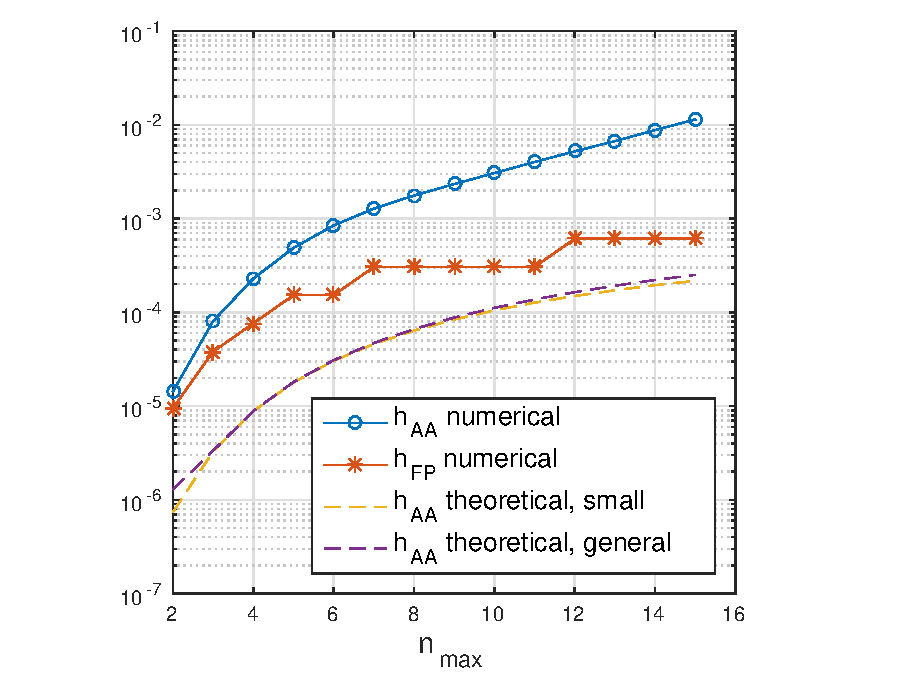
\includegraphics[width=4in]{Pictures/hVSnmax}
\caption{Variation of the step size with respect to the maximum number of iterations AA and FP are allowed to perform. Comparison between the theoretical estimations (\ref{eq:fullestimation}),(\ref{eq:lin_est}) and the numerical values.}
\label{fig:hVSnmax}
\end{figure}

\end{subsection}
\end{section}

% NONLINEAR ===============================================================================================================================================
\begin{section}{Nonlinear systems of ODEs}\label{subsec:nonlin}
The linear case is of limited interest in practical application, so let us consider the general nonlinear problem as it is defined in (\ref{eq:ode})
\begin{equation*}
	\begin{cases}
		\textbf{y}'(t) = f(t,\textbf{y}(t)), \quad \textbf{y}\in\mathbb{R}^n, f: [0,\infty] \times \mathbb{R}^n \rightarrow \mathbb{R}^n,\\
		\textbf{y}(0) =  \textbf{y}_0.
	\end{cases}
\end{equation*}
In the following, a strategy to solve this problem numerically based on implicit Runge Kutta methods and AA will be presented, as well as the results of three different numerical experiments. Since the scope of this work is verifying the efficiency of AA, the nonlinear problems arising from the numerical integration are solved using AA. In particular, the algorithm defined at the beginning of this work is slightly changed in this frame. In fact, it is more relevant using AA with a maximum number of iterations that is large and that is only used to prevent stalling processes, using as an arresting criterion only the norm of the residual.

% METHODS ===============================================================================================================================================
\begin{subsection}{The methods}
\textbf{Implicit Trapezoidal Rule (IT).} The first method chosen to compute the numerical solution of problem (\ref{eq:ode}) is IT, i.e. the $\theta$-method with $\theta = 0.5$. The method is defined at each time step by the following fixed point equation
\begin{equation*}
        y_{n+1}^{IT} = \phi_{IT}(y_{n+1}^{IT}; y_n, h_n, f) = y_n + 0.5 \cdot h_n f(t_n,y_n) + 0.5 \cdot h_n f(t_{n}+h_{n},y_{n+1}^{IT}).
\end{equation*} This method is known to have an accuracy of second order and to be $A$-stable, so it does not have time step restrictions for any problem. It is also true that IT is not $L$-stable, which means that for stiff problem it can produce oscillations, which usually tend to decrease in amplitude as the stiff part of the problem is over, but which are an additional source of error on the solution. \\

\textbf{Radau IIA (RIIA).} Another implicit method which is chosen to test the performances of AA is the RIIA. This is a collocation method defined by the following Butcher table
\begin{equation*}
\begin{array}{l | c c}
      \rule{0pt}{2,3ex} 1/3     &     5/12      &     -1/12    \\
      \rule{0pt}{2,3ex} 1       &     3/4       &      1/4     \\ [1,0ex] \hline
      \rule{0pt}{2,3ex}         &     3/4 	&      1/4
\end{array}.
\end{equation*}
For this method the fixed point equation is slightly different from the ones which have already been mentioned in this work. In fact, this method has two stages, so the fixed point solution is a vector consisting of all the internal stages. The definition of the problem is then
\begin{equation}\label{eq:radaufp}
\begin{split}
	z_{n+1} &= \begin{pmatrix} k_1 \\ k_2 \end{pmatrix} = \phi_{RIIA}(z_{n+1}; y_n, h_n, f) \\
		&= \begin{pmatrix} f(t_n + 1/3h_n,y_n + h_n(5/12k_1 - 1/12k_2)) \\ f(t_n+h_n,y_n + h_n(3/4k_1 + 1/4k_2)) \end{pmatrix}, \quad k_1,k_2 \in \mathbb{R}^n,          
\end{split}
\end{equation}
where $n$ is the size of the system. Finally
\begin{equation*}
	y_{n+1}^{RIIA} = y_{n} + 3/4k_1 + 1/4k_2.
\end{equation*}
Since this method is a Radau method on two stages, it is a method of third order. Furthermore, as all Radau methods, it is both $A$-stable and $L$-stable, which means that it does not have time step restrictions and that it suits well for stiff problems as well. \\

\textbf{Runge Kutta Chebyshev (RKC).} The third method chosen for verifying the efficiency of AA in a Runge Kutta frame is RKC. This method, based on Chebyshev polynomials, is the main example of an explicit method with extended stability. Given a step size $h_n$, the value of the solution at the previous time $y_n$ and an integer number of stages $s$, the method is defined as 
\begin{align*}
	&g_0 = y_n, \\
	&g_1 = y_n + \frac{h}{s^2} f(y_n),\\
	&g_i = \frac{2h}{s^2}f(g_{i-1}) + 2g_{i-1} - g_{i-2}, \quad i = 2,\dots,s, \\
	&y_{n+1}^{RKC} = g_s.
\end{align*}
As it was mentioned before this method is explicit, so it does not require any solver of nonlinear equations to compute $y_{n+1}$. Hence, RKC will be used only as a matter of comparison with the methods IT and RIIA when AA is used to compute the solution. The choice of RKC is due to the fact that it has an extended stability domain, and it suits well for problems characterized by eigenvalues with a large negative real part. It can be shown that the following step size restriction holds
\begin{equation}\label{eq:RKC}
	h \in \mathbb{R} \colon 0 \leq h \leq \frac{2s^2}{\rho},
\end{equation}
where $\rho$ is the spectral radius of the Jacobian of $f$ and $s$ is the chosen number of stages. The good stability behaviour of this method is given by the fact that the stability region increases quadratically with respect to the number of stages. As far as accuracy is concerned, this method is of first order. \\

\textbf{Runge Kutta Chebyshev, second order (RKCII).} The last method considered in this work is the RKCII, a Runge Kutta Chebyshev method of second order. As far as stability is concerned, this method has features similar to RKC, but in terms of accuracy it is of second order, so it provides a better comparison with IT on the basis of their performances. The algorithm defining this method and further theoretical results could be found in \cite{HW}.
\end{subsection}

% STRATEGY ===============================================================================================================================================
\begin{subsection}{Error estimation}\label{subsec:errorestim}
When an estimation of the error is needed in order to build an adaptive scheme, it is a common technique to let two Runge Kutta methods of different order compute the solution of the same problem on the same integration points. Let us denote by $y_n$ and $\tilde{y}_n$ the two different numerical solutions at time step $t_n$, and by $p$ and $\tilde{p}$ the orders of the two methods, with $\tilde{p} < p$. The local error at time step $t_n$ will then be 
\begin{equation*}
	err_n = \|y_{n} - \tilde{y}_{n}\| \leq \|y_{n} - y(t_{n})\| + \|y(t_{n}) - \tilde{y}_{n}\| = O(h^{\tilde{p}+1})
\end{equation*} 
where $y(t_{n})$ is the exact solution computed at time $t = t_{n}$. In the case of IT and RIIA, the solution which is computed in parallel is given by IE. The numerical solution of IE is given by the solution of the following fixed point problem 
\begin{equation*}
	y_{n+1}^{IE} = \phi_{IE}(y_{n+1}^{IE}; y_n, h_n, f) = y_n + h_n f(t_{n+1},y_{n+1}^{IE}). \\
\end{equation*}
In order to obtain an exhaustive idea of its performances, this solution is computed using AA as well. It is known that IE has order of accuracy 1, so the following local estimations are true
\begin{equation*}
\begin{aligned}
	err_{n+1}^{IT} = \|y_{n+1}^{IT} - y_{n+1}^{IE}\| = O(h^{2}), \\
	err_{n+1}^{RIIA} = \|y_{n+1}^{RIIA} - y_{n+1}^{IE}\| = O(h^{2}),
\end{aligned}
\end{equation*}
Since IE is the one-stage Radau method, it is known that it is both $A$-stable and $L$-stable, so it does not either diverge or oscillate spoiling the error estimation.
\end{subsection}

\begin{subsection}{Adaptivity}\label{sect:adapt}
Considering IT and RIIA, it is possible to apply an adaptivity procedure for the step sizes. In particular, once an estimation of the error $err_n$ is available at time step $t_n$, if it is bigger than the tolerance the current step size $h_n$ is refused and the following step size is used starting from $t_n$
\begin{equation*}
	h_{new} = h_n \cdot \Big{(}\frac{tol}{err_n}\Big{)}^{1/(\tilde{p}+1)},
\end{equation*}
where $\tilde{p}$ is defined as in section \ref{subsec:errorestim}. In this case $\tilde{p} = 1$, since it is the order of IE. If the error $err_n$ is smaller than the tolerance $tol$, the step size is accepted and the step size $h_{n+1}$ is chosen as
\begin{equation*}
	h_{n+1} = h_n \cdot \Big{(}\frac{tol}{err}\Big{)}^{1/(\tilde{p}+1)}.
\end{equation*}
\end{subsection}

\begin{subsection}{Runge Kutta Chebyshev Strategy}\label{subsec:RKCstrat}
The previous procedure for estimating the error and adapting the step size is used in this work only for IT and RIIA, while for RKC and RKCII the procedure is different. In fact, the solution given by those two methods is computed using a fixed step size, while the number of stages is adapted in order to ensure stability. Indeed, if we dispose of the Jacobian associated to the system of ODEs, it is possible to estimate the number of stages sufficient to ensure stability. At the time $t_n$ this estimate is given by
\begin{equation*}
	s_n = \left \lceil{\sqrt{ \frac{1}{2}h|\lambda_{max}(t_n)|}}\right \rceil,
\end{equation*}
where $h$ is the step size and $\lambda_{max}(t_n)$ is the maximum eigenvalue of the Jacobian in absolute value at time $t_n$. The ceil operator is applied since the number of stages has to be an integer.
\end{subsection}

\begin{subsection}{Computational cost}
Being the scope of this work studying the efficiency of AA in a Runge Kutta frame, it is important keeping track of the computational work needed in order to compute the numerical solution. Since all the code of this work is implemented in \texttt{Matlab}, using the computational time as a matter of comparison is not a reasonable choice. Hence, comparing the number of function evaluations needed for the integration represents a more suitable strategy. For the implicit methods (IE, IT and RIIA) the function evaluations are computed only inside AA. If the methods are implemented carefully the number of function evaluations at each time step is equal to the number of stages of the Runge Kutta method (one for IE and IT, two for RIIA) multiplied by the number of iterations performed by AA, as in the following
\begin{equation*}
	\#f.ev_n(RK) = \#iterations(AA)_n \cdot \#stages(RK), \quad n = 1,2,\dots \; .
\end{equation*}
Hence, globally the number of function evaluations is equal to the sum over the accepted and refused time steps of the above quantity. It is clear that since at each time step an estimation of the error is required by the method, the number of function evaluations is equal to the sum of the two method that run in parallel. So, for the two considered method (IT and RIIA), with IE used to estimate the error, it is clear that 
\begin{align*}
	\#f.ev_n(IT + IE) &= 2\cdot\#iterations(AA)_n, \\
	\#f.ev_n(RIIA + IE) &= 3\cdot\#iterations(AA)_n.
\end{align*}
For RKC and RKCII the computational cost is instead given locally by 
\begin{equation*}
	\#f.ev_n(RKC) = s_n, \quad n = 1,2,\dots,
\end{equation*}
where $s_n$ is the number of stages performed at time $t_n$. The global computational cost is then given by the sum over the time steps of the above local quantity.
\end{subsection}

% NUMERICAL EXPERIMENTS ===============================================================================================================================================
\begin{subsection}{Numerical Experiments}
\textbf{BRUSS} As a first example, let us consider the Brusselator problem (BRUSS) \cite{HW}. The problem is defined as
\begin{equation*}
\begin{aligned}
	\frac{\partial u}{\partial t} &= A + u^2v - (B+1)u + \alpha \frac{\partial^2u}{\partial x^2}, \\
	\frac{\partial v}{\partial t} &= Bu - u^2v + \alpha \frac{\partial^2v}{\partial x^2},
\end{aligned}
\end{equation*}
where $0\leq x \leq 1, 0 \leq t \leq T, T = 10, A = 1, B = 3, \alpha = 1/50$ and the initial and boundary conditions are
\begin{equation*}
\begin{aligned}
	u(0,t) &= u(1,t) = 1,  &  v(0,t) = v(1,t) = 3, \\
	u(x,0) &= 1 + 0.5\sin(2\pi x), &  v(x,0) = 3.
\end{aligned}
\end{equation*}
Discretizating this equation in space with the method of lines on
\begin{equation*}
	x_i = i/(N+1), \quad 1 \leq i \leq N, \quad \Delta x = 1/(N+1),
\end{equation*}
it is possible to obtain the following system of ODEs of size $n = 2N$
\begin{equation}\label{eq:BRUSS}
\begin{aligned}
	u_i &= 1 + u_i^2v_i - 4u_i + \frac{\alpha}{\Delta x^2}(u_{i-1} - 2u_{i} + u_{i+1}), i = 1,\dots,N,\\
	v_i &= 3u_i - u_i^2v_i + \frac{\alpha}{\Delta x^2}(v_{i-1}-2v_i + v_{i+1}), i = 1,\dots,N,
\end{aligned}
\end{equation}
where the initial and boundary conditions are retrieved by imposing
\begin{equation*}
\begin{aligned}
	u_0(t) &= u_{N+1}(t) = 1,  &  v_0(t) = v_{N+1}(t) = 3, \\
	u_i(0) &= 1 + 0.5\sin(2\pi x_i), & v_i(0) = 3, \quad i = 1,\dots,N.
\end{aligned}
\end{equation*}
This equation is stiff for big values of $N$. In particular, the value chosen for this experiment is $N = 500$. In Figure \ref{fig:BRUSSsol} the approximate solution $u(t,x)$ for $N = 20$ obtained using RIIA with the strategy described above with a tolerance $10^{-2}$ is shown.
\begin{figure}[t!]
\centering
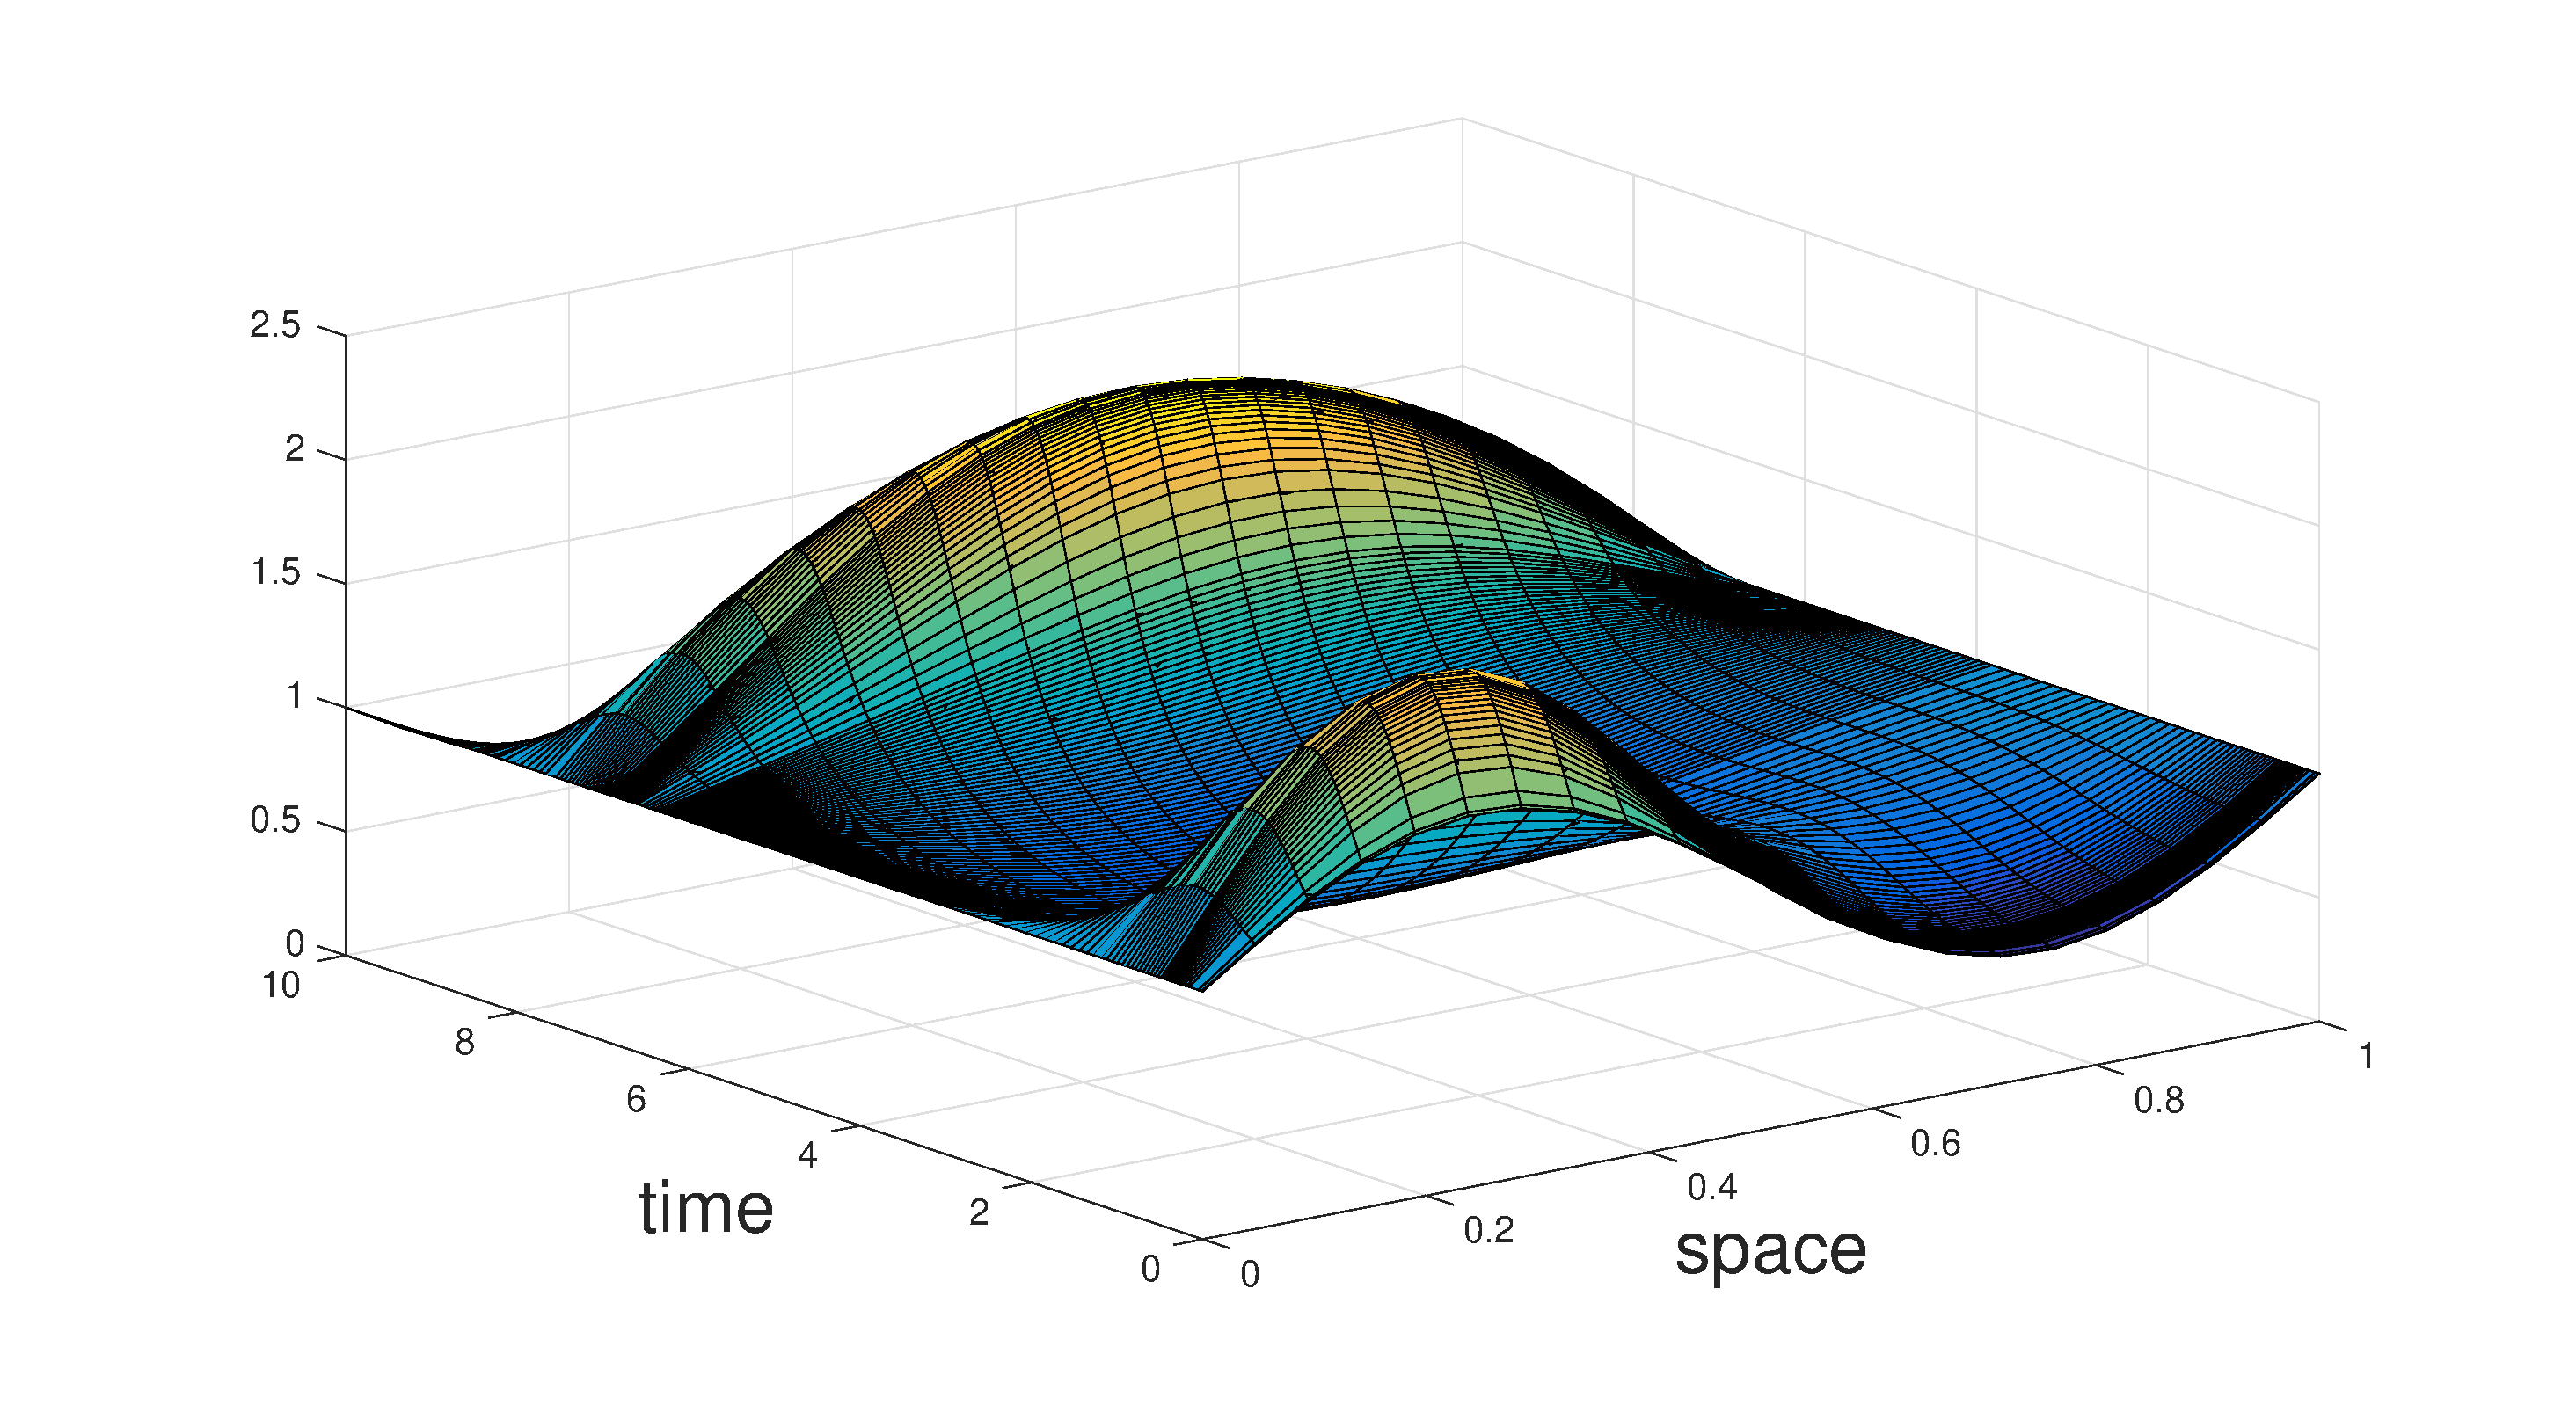
\includegraphics [width=4in]{Pictures/BRUSSNICE.eps}\\
\caption{Solution $u(t,x)$ of the Brussellator for $N = 20$ with RIIA and tolerance $10^{-2}$.}
\label{fig:BRUSSsol}
\end{figure}
The aim is then comparing the different methods in terms of efficiency and accuracy on the exact solution using an \textit{err-work} plot. The numerical solution is computed using IT and RIIA for $N = 500$ and for different values of the tolerances. In particular, the values chosen are $tol_j = 10^{-j}, j = 2,\dots,7$. Then the error is computed at final time $T = 10$ using as a reference solution the one from \cite{JC}. The chosen norm for the error is the Euclidean norm
\begin{equation}\label{eq:err}
	\|y_{k} - y(T)\| = \sqrt{\sum_{i = 1}^N(y_{k,i} - y_i(T))^2}, \quad k \in \mathbb{R} \colon t_k = T,
\end{equation}
where the index $i$ refers to the components of the numerical and the exact solution. As for RKC and RKCII, the solution is computed with different fixed time steps as described in section \ref{subsec:RKCstrat}. In particular, for this experiment the chosen time steps are $h_j = 10^{-j}, j = 1,\dots,7$. The obtained results are shown in the logarithmic scale plot of Figure \ref{fig:BRUSSres}. In the plot the bold circles refer to the value of tolerance $10^{-5}$ for the two implicit methods and to the step size $10^{-5}$ for RKC and RKCII.
\begin{figure}[t!]
\centering
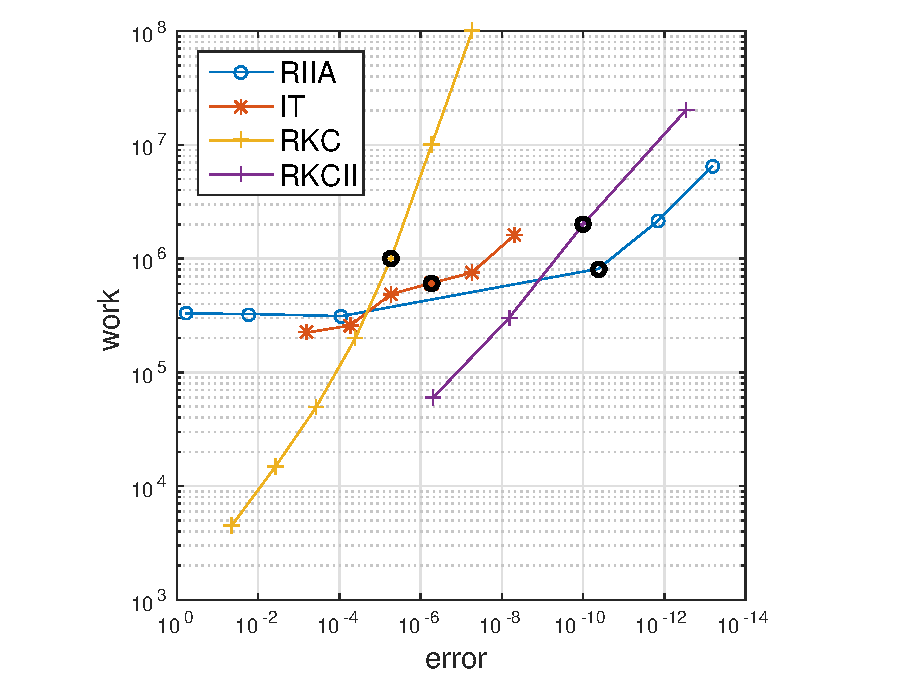
\includegraphics [width=4in]{Pictures/BRUSSresults.eps}
\caption{err-work plot of the Brussellator problem.}
\label{fig:BRUSSres}
\end{figure}
Let us comment the results. As far as RKC is concerned, it is clear from the strategy explained in section \ref{sect:adapt} that refining the step size the number of function evaluations increase practically at the same rate. It is furthermore possible to observe that the error dicreases linearly with the step size. RKCII gives better results than RKC due to its higher order, as the error dicreases quadratically with the step size. The IT method gives acceptable results as well. All the error values are around one order of magnitude below their associated tolerance, and the number of function evaluations is reasonable with respect to the other methods. It is in fact possible to see that the err-work curve of IT is below the one associated to RKC from the value of tolerance $10^{-5}$ and for all the smaller values, but, on the other hand, it is also true that RKCII requires less function evaluations in order to obtain an error of the same order of magnitude. The behaviour of RIIA is of difficult interpretation. It is possible to remark that for the higher values of the tolerances, i.e., $10^{-2},10^{-3}$, the solution does not even meet the accuracy requirement, as the error value is bigger than it. For $10^{-4}$ the result is similar to the result of IT, but for the smaller values, i.e., $10^{-5},10^{-6},10^{-7}$, the solution is much more accurate than the required tolerance, as the error values are all below $10^{-10}$, with a number of function evaluations which lays between IT and RKC.\\

\textbf{HIRES} Let us consider the HIRES chemical reaction \cite{HW}. The problem is defined by the following system of ODEs of dimension 8
\begin{equation}\label{eq:HIRES}
\begin{aligned}
	y_1' &= -1.71y_1 + 0.43y_2 + 8.32y_3 + 0.0007, \\
	y_2' &= 1.71y_1 -8.75y_2, \\
	y_3' &= -10.03y_3 + 0.43y_4 + 0.035y_5, \\
	y_4' &= 8.32y_2 + 1.71y_3-1.12y_4, \\
	y_5' &= -1.745y_5 + 0.43y_6 + 0.43y_7, \\
	y_6' &= -280y_6y_8 + 0.69y_4 + 1.71y_5 - 0.43y_6 + 0.69y_7, \\
	y_7' &= 280y_6y_8 - 1.81y_7, \\
	y_8' &= -y_7',
\end{aligned}
\end{equation} 
integrated in the time span $0 \leq t \leq 321.8122$ and endowed with the following initial conditions
\begin{equation*}
	y_1(0) = 1, \quad y_2(0) = y_3(0) = \dots = y_7(0) = 0, \quad y_8(0) = 0.0057.
\end{equation*}
This problem is not very stiff and ``can also be solved by explicit methods''\cite{HW}. In fact, thanks to this feature this problem is good for comparing the solution provided by IT with the solution provided by RKC and RKCII in terms of accuracy and work. The chose tolerances are the same as in BRUSS, i.e. $tol_j = 10^{-j}, j = 2,\dots,7$. As far as RKC is concerned, because of the length of the interval and of the low stiffness of the problem, the chosen step sizes are $h_j = 10^{-j}, j = 1,\dots,6$, while for RKCII the step sizes are $h_j = 10^{-j}, j = 2,\dots,6$. For smaller step sizes the problem is not practical to solve, since as RKC requires at least one function evaluation at each time step, this implementation of the method would be not optimal at all. The numerical solutions are then compared at the final time with the exact solution provided in \cite{HAIR}, computing the error as in (\ref{eq:err}). The results are shown in Figure \ref{fig:HIRES} , where the bold circle in this case indicates the solution given by IT with the tolerance $10^{-5}$ and the one given by RKC and RKCII with the step size $10^{-3}$.
\begin{figure}[t!]
\centering
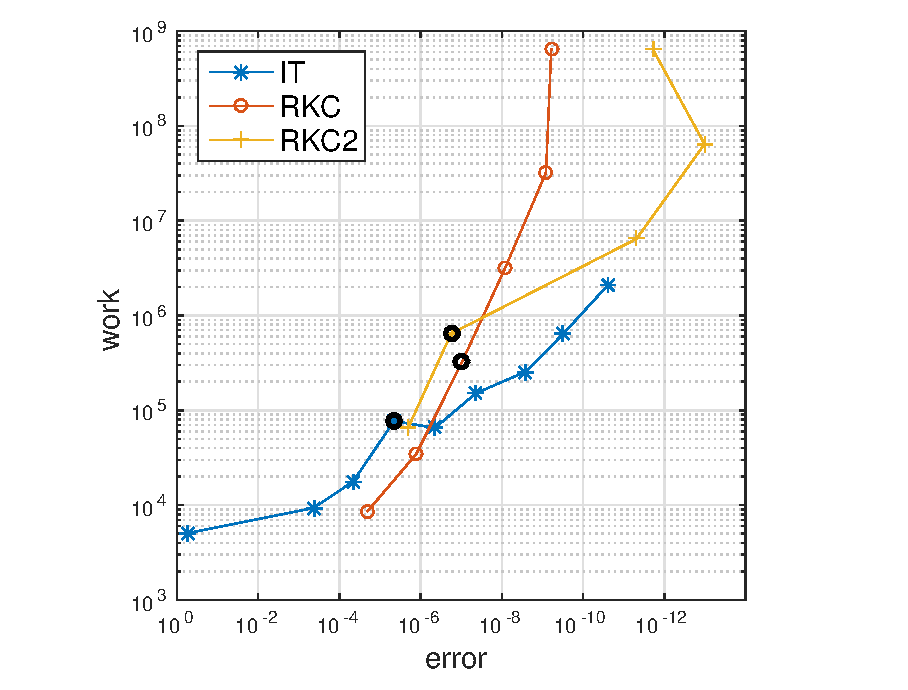
\includegraphics [width=4in]{Pictures/HIRES.eps}
\caption{err-work plot of the HIRES reaction.}
\label{fig:HIRES}
\end{figure}
It is possible to remark that the IT method performs well in this case. The error given by the tolerance $10^{-1}$ is not satisfactory, but the other values for the error are acceptable with respect to their tolerance. Moreover, IT is competitive with both RKC and RKCII in terms of computational cost, as for similar values of the error the number of function evaluations is comparable. In fact, for small error values on the exact solution, IT performs less function evaluations than the Runge Kutta Chebyshev methods.\\

\textbf{VDPOL} The last problem considered in this work is the Van der Pol oscillator \cite{HW}. It is defined as follows
\begin{equation}\label{eq:VDPOL}
\begin{aligned}
	y_1' &= y_2, \\
	y_2' &= ((1 - y_1^2)y_2 - y_1)/\epsilon, \quad \epsilon = 10^{-6},
\end{aligned}
\end{equation} 
integrated in the time span $0 \leq t \leq 1$ and endowed with the following initial conditions
\begin{equation*}
	y_1(0) = 2, \quad y_2(0) = 0.
\end{equation*}
This problem is a typical example of a ``very stiff problem of small dimension''\cite{HW}. It is in fact the example which requires the highest cost among the ones considered in this work, even though it consists only of two equations. In this case the eigenvalues of the Jacobian do not possess a particularly large negative real part, but on the other side they have a large imaginary part. This causes fast oscillations in the solution, which makes it practically impossible to find it numerically using RKC or RKCII, as those methods are used to integrate equations mainly characterized by negative real eigenvalues. In Figure \ref{fig:VDPOL} it is possible to see the \textit{err-work} plot relative to IT with values of tolerances $10^{-i},i=2,\dots,6$. As usual, the bold circle is relative to the tolerance $10^{-5}$.
\begin{figure}[t!]
\centering
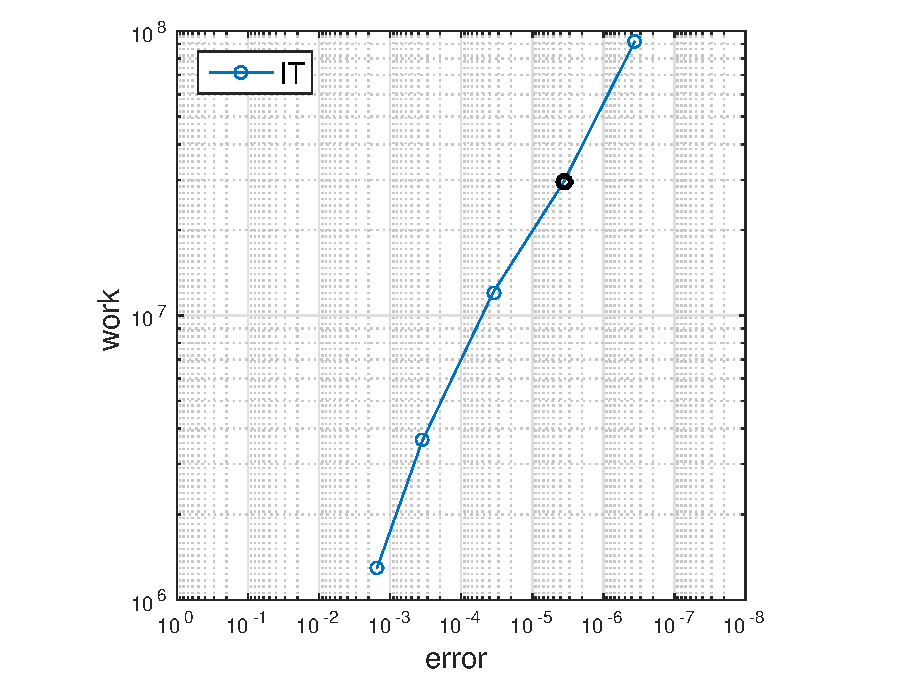
\includegraphics [width=4in]{Pictures/VDPOL.eps}
\caption{err-work plot of the Van der Pol oscillator.}
\label{fig:VDPOL}
\end{figure}
Let us remark that for similar values of the error, the number of function evaluations is of one order of magnitude higher than the same values for BRUSS and of two order of magnitudes higher than HIRES. Therefore, it has been difficult integrating this equation due to the high computational time, and the only code which gave acceptable results is IT. In any case, the error values are all acceptable with respect to the required tolerances. The accepted step sizes, as represented in Figure \ref{fig:VDPOL_stps}, show both the oscillating behaviour of the solution and the dramatic decrease of their value in correspondence to the time instant in which the equation is mostly stiff.
\begin{figure}[t!]
\centering
\includegraphics [width=4in]{Pictures/VDPOL_stepsize.eps}
\caption{step sizes selected by IT for integrating the Van der Pol oscillator for $tol = 10^{-6}$.}
\label{fig:VDPOL_stps}
\end{figure}
\end{subsection}
\end{section}

% CONCLUSION ===============================================================================================================================================
\begin{section}{Conclusion}
In this work we have analyzed the features of the Anderson Acceleration method for nonlinear system of equations. In particular, we have tested its performances when it is used to solve the fixed point problem defined by an implicit Runge Kutta method. We have focused especially on stiff systems of equations, since they have to be integrated using implicit methods. The Anderson Acceleration method does not require the solution of linear systems, unlike the classic Newton method, therefore explicit Runge Kutta methods with extended stability are a good matter of comparison for its performances in this frame. We noticed that implicit methods implemented with Anderson Acceleration are competitive with the Runge Kutta Chebyshev methods, especially when integrating problems which are not particularly stiff over a long time, such as the HIRES chemical reaction.

\end{section}

\clearpage
\bibliographystyle{siam}
\bibliography{Biblio}{}
\end{document}

\grid
